\documentclass[tikz,border=10pt]{standalone}
\usepackage{tikz}
\usetikzlibrary{mindmap,trees}

\tikzset{
  cloudnative mindmap/.style={
    mindmap,
    grow cyclic,
    every node/.style=concept,
    concept color=black!10,
    level 1/.append style={
      level distance=5.5cm,
      sibling angle=72,
      font=\bfseries\small,
    },
    level 2/.append style={
      level distance=3.8cm,
      sibling angle=40,
      font=\scriptsize,
    },
  }
}

\begin{document}

\newcommand{\mindmap}[5]{
\node [concept, concept color=black!70, text=white, font=\bfseries\normalsize]
  {Cloud-Native\\Landscape}
  child [concept color=#1] { node {Provisioning}
    child { node {Automation \&\\Configuration} }
    child { node {Container\\Registry} }
    child { node {Security \&\\Compliance} }
    child { node {Key\\Management} }
  }
  child [concept color=#2] { node {Runtime}
    child { node {Cloud-native\\Storage} }
    child { node {Container\\Runtime} }
    child { node {Cloud-native\\Network} }
  }
  child [concept color=#3] { node {Orchestration \&\\Management}
    child { node {Scheduling \&\\Orchestration} }
    child { node {Coordination \&\\Service Discovery} }
    child { node {Remote\\Procedure Call} }
    child { node {Service\\Proxy} }
    child { node {API\\Gateway} }
    child { node {Service\\Mesh} }
  }
  child [concept color=#4] { node {App Definitions \&\\Development}
    child { node {Database} }
    child { node {Streaming \&\\Messaging} }
    child { node {App Definition \&\\Image Build} }
    child { node {CI \& CD} }
  }
  child [concept color=#5] { node {Observability \&\\Analysis}
    child { node {Observability} }
    child { node {Chaos\\Engineering} }
  }
;  
}

% \begin{tikzpicture}[
% cloudnative mindmap]

% \node [concept, concept color=black!70, text=white, font=\bfseries\normalsize]
%   {Cloud-Native\\Landscape}
%   child [concept color=blue!60] { node {Provisioning}
%     child { node {Automation \&\\Configuration} }
%     child { node {Container\\Registry} }
%     child { node {Security \&\\Compliance} }
%     child { node {Key\\Management} }
%   }
%   child [concept color=green!55!black] { node {Runtime}
%     child { node {Cloud-native\\Storage} }
%     child { node {Container\\Runtime} }
%     child { node {Cloud-native\\Network} }
%   }
%   child [concept color=orange!80!black] { node {Orchestration \&\\Management}
%     child { node {Scheduling \&\\Orchestration} }
%     child { node {Coordination \&\\Service Discovery} }
%     child { node {Remote\\Procedure Call} }
%     child { node {Service\\Proxy} }
%     child { node {API\\Gateway} }
%     child { node {Service\\Mesh} }
%   }
%   child [concept color=red!65] { node {App Definitions \&\\Development}
%     child { node {Database} }
%     child { node {Streaming \&\\Messaging} }
%     child { node {App Definition \&\\Image Build} }
%     child { node {CI \& CD} }
%   }
%   child [concept color=violet!70] { node {Observability \&\\Analysis}
%     child { node {Observability} }
%     child { node {Chaos\\Engineering} }
%   }
% ;
% \end{tikzpicture}


\begin{tikzpicture}[
  cloudnative mindmap]
  \label{page:devops:cloudnative_mm:full}
  \mindmap{blue!60}{green!55!black}{orange!80!black}{red!65}{violet!70}
\end{tikzpicture}

\begin{tikzpicture}[
  cloudnative mindmap]
  \label{page:devops:cloudnative_mm:provisioning}
  \mindmap{blue!60}{white}{white}{white}{white}
\end{tikzpicture}

\begin{tikzpicture}[
  cloudnative mindmap]
  \label{page:devops:cloudnative_mm:runtime}
  \mindmap{white}{green!55!black}{white}{white}{white}
\end{tikzpicture}

\begin{tikzpicture}[
  cloudnative mindmap]
  \label{page:devops:cloudnative_mm:orchestration}
  \mindmap{white}{white}{orange!80!black}{white}{white}
\end{tikzpicture}

\begin{tikzpicture}[
  cloudnative mindmap]
  \label{page:devops:cloudnative_mm:appdef}
  \mindmap{white}{white}{white}{red!65}{white}
\end{tikzpicture}

\begin{tikzpicture}[
  cloudnative mindmap]
  \label{page:devops:cloudnative_mm:observe}
  \mindmap{white}{white}{white}{white}{violet!70}
\end{tikzpicture}



% alternative: reduced layout
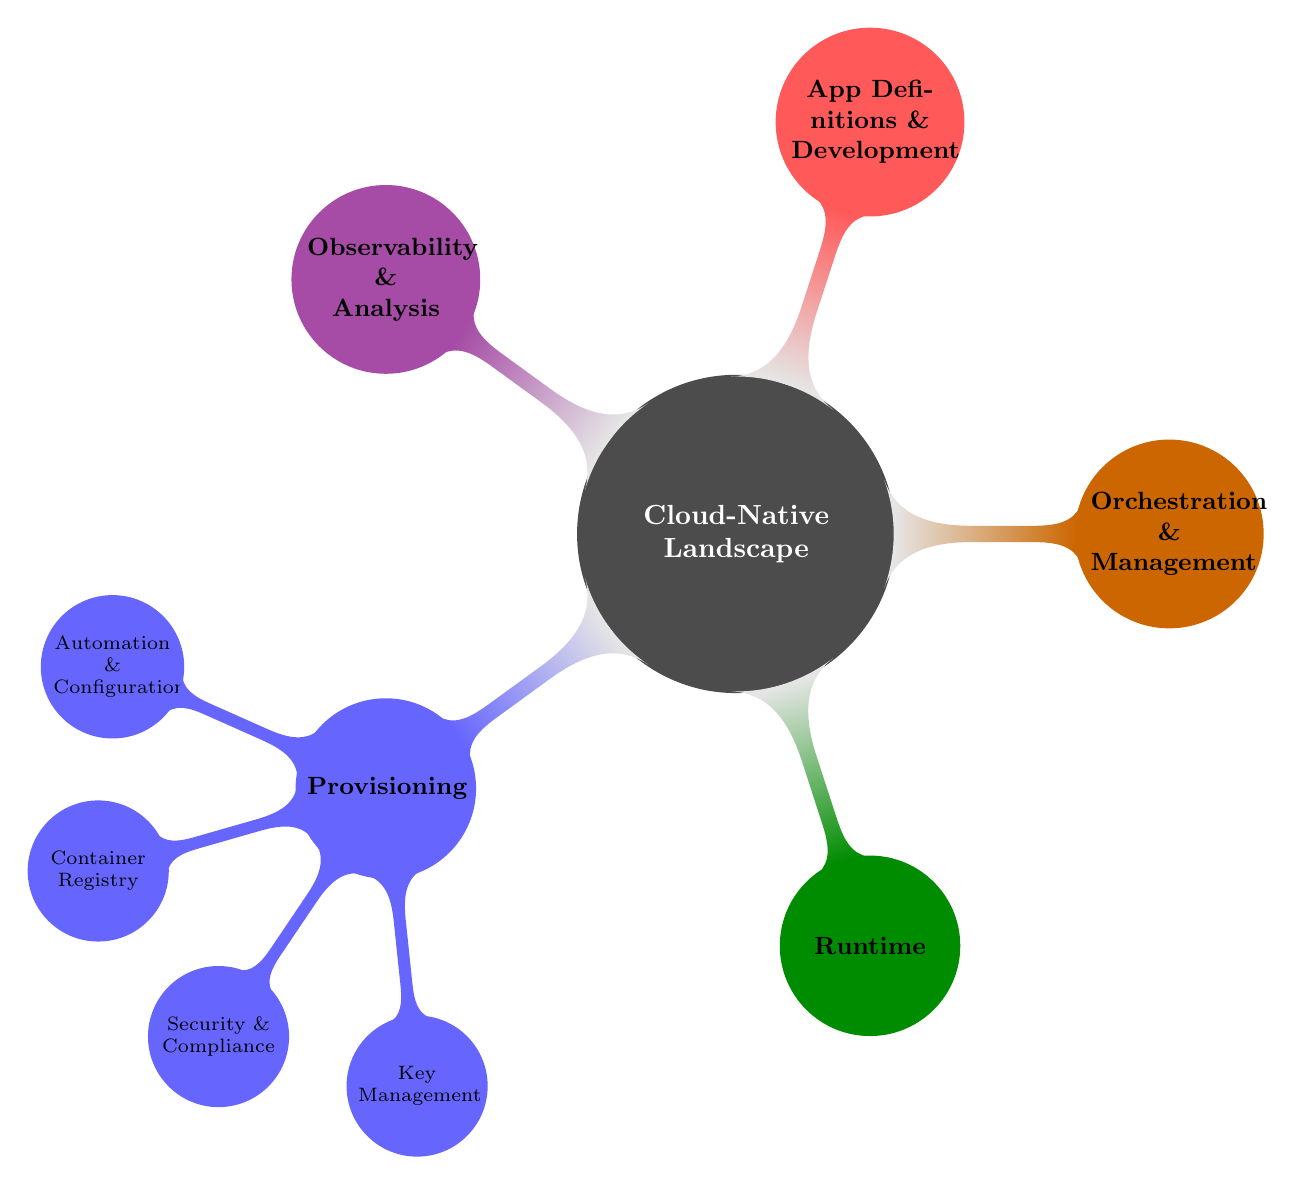
\begin{tikzpicture}[
  cloudnative mindmap,
]

\node [concept, concept color=black!70, text=white, font=\bfseries\normalsize]
  {Cloud-Native\\Landscape}
  child [concept color=blue!60] { node {Provisioning}
    child { node {Automation \&\\Configuration} }
    child { node {Container\\Registry} }
    child { node {Security \&\\Compliance} }
    child { node {Key\\Management} }
  }
  child [concept color=green!55!black] { node {Runtime}
  }
  child [concept color=orange!80!black] { node {Orchestration \&\\Management}
  }
  child [concept color=red!65] { node {App Definitions \&\\Development}
  }
  child [concept color=violet!70] { node {Observability \&\\Analysis}
  }
;
\end{tikzpicture}

\end{document}
